\documentclass{standalone}
\usepackage{tikz}
\usetikzlibrary{shadows}
\def\F{\mathsf{F}} % in future
\def\G{\mathsf{G}} % globally

\begin{document}

\def\mycyan{cyan!30}
\def\mypink{magenta!30}
\scalebox{1.2}{
 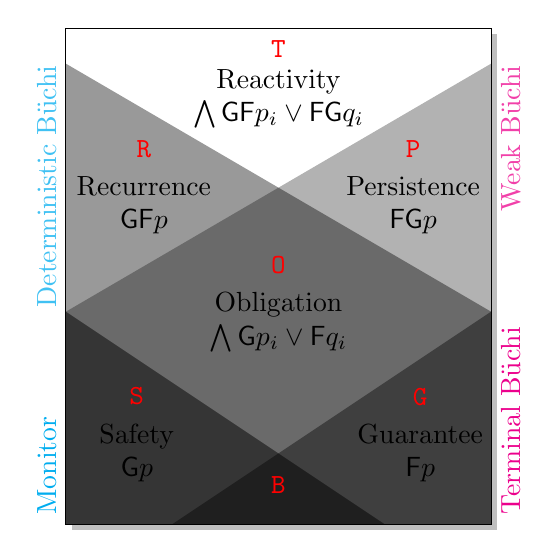
\begin{tikzpicture}[scale=.9]
    \draw[drop shadow,fill=white] (0,0) rectangle (6,7);

    \path[fill=\mycyan,fill opacity=.4] (0,6.5) -- (6,3) -- (6,0) -- (0,0);
    \path[fill=\mycyan,fill opacity=.5] (0,3) -- (4.5,0) -- (0,0);
    \path[fill=\mypink,fill opacity=.3] (6,6.5) -- (0,3) -- (0,0) -- (6,0);
    \path[fill=\mypink,fill opacity=.4] (6,3) -- (1.5,0) -- (6,0);
    \draw (0,0) rectangle (6,7);

    \node[align=center] (rea) at (3,6) {Reactivity\\ $\bigwedge\G\F p_i\lor \F\G q_i$};
    \node[align=center] (rec) at (1.1,4.5) {Recurrence\\ $\G\F p$};
    \node[align=center] (per) at (4.9,4.5) {Persistence\\ $\F\G p$};
    \node[align=center] (obl) at (3,2.85) {Obligation\\ $\bigwedge\G p_i\lor \F q_i$};
    \node[align=center] (saf) at (1,1) {Safety\\ $\G p$};
    \node[align=center] (gua) at (5,1) {Guarantee\\ $\F p$};

    \node[above left,rotate=90,color=cyan!75] (det) at (0,6.5) {Deterministic B\"uch\rlap{i}};
    \node[above right,rotate=90,color=cyan](weak) at (0,0) {Monitor};
    \node[below left,rotate=90,color=magenta!75](weak) at (6,6.5) {Weak B\"uch\rlap{i}};
    \node[below right,rotate=90,color=magenta](weak) at (6,0) {Terminal B\"uchi};

    \node[above=-1mm,red] at (rea.north) {\tt T};
    \node[above,red] at (rec.north) {\tt R};
    \node[above,red] at (per.north) {\tt P};
    \node[above,red] at (obl.north) {\tt O};
    \node[above,red] at (saf.north) {\tt S};
    \node[above,red] at (gua.north) {\tt G};
    \node[above,red] at (3,0.3) {\tt B};
  \end{tikzpicture}}
\end{document}
%%% Local Variables:
%%% mode: latex
%%% TeX-master: t
%%% End:
